\chapter{Testbench}
\begin{figure}[h!]
	\centering
	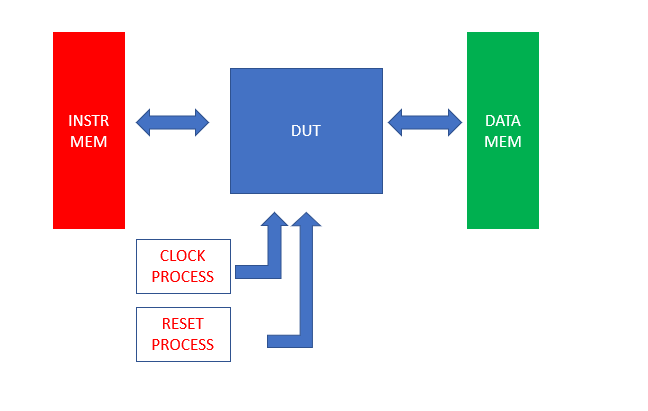
\includegraphics[width=10cm]{./images/Testbench}
	\caption{Testbench organizatiopn}
	\label{fig4.1}
\end{figure} 
The Clock process generate the clock signal for the entire processor.\\
We have decided to adopt a 20ns as a period for the testbench.\\
So our processor is tested at 50MHz. \\
Our goal was to verify that the processor works correctly, withouth considering the performance. \\
For this reason we have used a low frequency.\\
The reset process initialize all the component. This signal is active for 15ns then it is disabled.\\
For what concern the Instruction and Data memory we have implemented both like array of 32 bits.\\
This because both memory are not so big, we have decided to implement them without resorting to a specific structure.\\
\begin{figure}[h!]
	\centering
	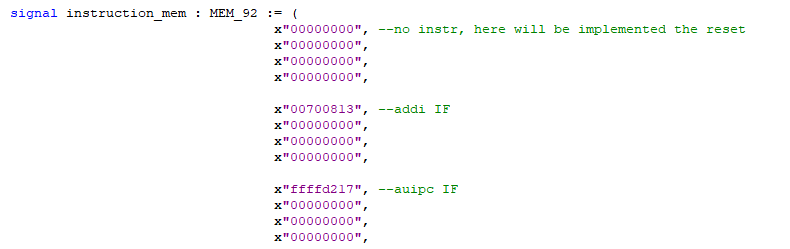
\includegraphics[width=18cm]{./images/Imem}
	\caption{Memory example}
	\label{fig4.2}
\end{figure} 
So for the Instruction memory we have taken the program to test the architecture(Given in the specification)\\
and we have written all the instruction manually. All of them are interleaved by 3 empty instruction, to respect the\\
program counter update(PC+4).
The results are written in the Register file or in the Data memory, depending on which instruction is executed.

